\documentclass[12pt]{article}

\usepackage{amsmath, amssymb, amsthm, enumerate, graphicx}
\usepackage[usenames,dvipsnames]{color}
\usepackage{bm}
\usepackage[colorlinks=true,urlcolor=blue]{hyperref}
\usepackage{geometry}
\geometry{margin=1in}
\usepackage{float}
\usepackage{graphics}
\setlength{\marginparwidth}{2.15cm}
\usepackage{booktabs}
\usepackage{enumitem}
\usepackage{epsfig}
\usepackage{setspace}
\usepackage{parskip}
\usepackage[normalem]{ulem}
\usepackage{tikz}
\usetikzlibrary{positioning, arrows, automata}
\usepackage{pgfplots}
\usepackage[font=scriptsize]{subcaption}
\usepackage{float}
\usepackage[]{algorithm2e}
\usepackage{environ}
\usepackage{bbm}
\usepackage{graphicx}
\usepackage{titling}
\usepackage{url}
\usepackage{xcolor}
\usepackage{lipsum}
\usepackage{lastpage}
\usepackage[colorlinks=true,urlcolor=blue]{hyperref}
\usepackage{multicol}
\usepackage{tabularx}
\usepackage{comment}
\usepackage[utf8]{inputenc}
\usepackage{amssymb}
\usepackage{setspace}
\usepackage{marvosym}
\usepackage{wrapfig}
\usepackage{datetime}
\usepackage[many]{tcolorbox}
\usepackage{array}
\usepackage{multirow}
\usepackage{wasysym}
\usepackage{cancel}

\usepackage{listings}
\usepackage{color}
\usepackage[thinlines]{easytable}
\usepackage{lastpage}

\newcommand{\R}{\mathbb{R}}
\newcommand{\blackcircle}{\tikz\draw[black,fill=black] (0,0) circle (1ex);}
\renewcommand{\circle}{\tikz\draw[black] (0,0) circle (1ex);}


\usetikzlibrary{positioning,calc}


%-------------------------------------------------------------------------------
% Custom commands
\usepackage{xcolor} %hilight
\newcommand{\hilight}[1]{\colorbox{yellow}{#1}}
%-------------------------------------------------------------------------------

%%BEGINSOLUTION
% To delete solutions from the TeX file, do:
% sed '/\%\%BEGINSOLUTION/,/\%\%ENDSOLUTION/d' main.tex > out.tex
%%ENDSOLUTION
\newtcolorbox[]{solution}[1][]{%
    breakable,
    enhanced,
    colback=white,
    title=Solution,
    #1
}
\begin{document}
\section*{}
\begin{center}
  \centerline{\textsc{\LARGE  Homework 5 Template}}
\end{center}

Use this template to record your answers for Homework 5.  Add your answers using \LaTeX and then save your document as a PDF to upload to Gradescope.  You are required to use this template to submit your answers.  \textbf{You should not alter this template in any way} other than to insert your solutions.  You must submit all \pageref{LastPage} pages of this template to Gradescope.  Do not remove the instructions page(s).  Altering this template or including your solutions outside of the provided boxes can result in your assignment being graded incorrectly.

You should also export your code as a .py file and upload it to the \textbf{separate} Gradescope coding assignment. Remember to mark all teammates on \textbf{both} assignment uploads through Gradescope.

\section*{Instructions for Specific Problem Types}

On this homework, you must fill in blanks for each problem. Please make sure your final answer is fully included in the given space.  \textbf{Do not change the size of the box provided.}  For short answer questions you should \textbf{not} include your work in your solution.  Only provide an explanation or proof if specifically asked.

\begin{quote}
\textbf{Fill in the blank:} What is the course number?

\begin{tcolorbox}[fit,height=1cm, width=4cm, blank, borderline={1pt}{-2pt},nobeforeafter]
    \begin{center}\huge10703\end{center}
    \end{tcolorbox}
\end{quote}

\newpage

\section*{Problem 0: Collaborators}
Enter your team members' names and Andrew IDs in the boxes below. If you worked in a team with fewer than three people, leave the extra boxes blank.

Name 1: \begin{tcolorbox}[fit,height=1cm, width=5cm, blank, borderline={1pt}{1pt},nobeforeafter]
    \begin{center}
    \vspace{3mm}
    \large{Andrew Jong}
    \end{center}
\end{tcolorbox}
Andrew ID 1: \begin{tcolorbox}[fit,height=1cm, width=5cm, blank, borderline={1pt}{1pt},nobeforeafter]
    \begin{center}
    \vspace{3mm}
    \large{ajong}
    \end{center}
\end{tcolorbox}
    \\
Name 2: \begin{tcolorbox}[fit,height=1cm, width=5cm, blank, borderline={1pt}{1pt},nobeforeafter]
    \begin{center}
    \vspace{3mm}
    \large{Gabe Olin}
    \end{center}
\end{tcolorbox}
Andrew ID 2: \begin{tcolorbox}[fit,height=1cm, width=5cm, blank, borderline={1pt}{1pt},nobeforeafter]
    \begin{center}
    \vspace{3mm}
    \large{golin}
    %solution
    \end{center}
\end{tcolorbox} \\
Name 3: \begin{tcolorbox}[fit,height=1cm, width=5cm, blank, borderline={1pt}{1pt},nobeforeafter]
    \begin{center}
    \vspace{3mm}
    \large{Mike Anoruo}
    \end{center}
\end{tcolorbox}
Andrew ID 3: \begin{tcolorbox}[fit,height=1cm, width=5cm, blank, borderline={1pt}{1pt},nobeforeafter]
    \begin{center}
    \vspace{3mm}
    \large{manoruo}
    %solution
    \end{center}
\end{tcolorbox} \\
\vspace{0.5cm}
\vspace{0.5cm}

\newpage
\section*{Problem 1: Model-Based Reinforcement Learning with PETS (105 pt)}
\subsection*{1.1 Model-based Predictive Control (25 pts)}

\subsection*{1.1.1 CEM (without MPC) with ground-truth dynamics (10 pt)}

Success percentage
\begin{tcolorbox}[fit,height=1cm, width=5cm, blank, borderline={1pt}{1pt},nobeforeafter, valign=center]
\begin{center}
    \large{80\%}
\end{center}
\end{tcolorbox}

\subsection*{1.1.2 Random sampling with ground-truth dynamics. (10 pt)}

Success percentage without MPC 
\begin{tcolorbox}[fit,height=1cm, width=5cm, blank, borderline={1pt}{1pt},nobeforeafter, valign=center]
\begin{center}
    \large{68\%}
\end{center}
\end{tcolorbox}

Success percentage with MPC 
\begin{tcolorbox}[fit,height=1cm, width=5cm, blank, borderline={1pt}{1pt},nobeforeafter, valign=center]
\begin{center}
    \large{84\%}
\end{center}
\end{tcolorbox}

How does the performance of random sampling performance compare to that of CEM?
\begin{tcolorbox}[fit,height=5em, width=40em, blank, borderline={1pt}{1pt},nobeforeafter, valign=center]
\begin{center}
CEM performs better than random sampling in my experiments. CEM without MPC achieved an 80\% success rate, while random sampling without MPC only reached 68\%. With MPC, random sampling improves to 84\%, but CEM still outperforms it. This shows CEM’s iterative refinement helps find better action sequences, leading to higher success rates compared to random sampling.
\end{center} 
\end{tcolorbox}

\subsection*{1.1.3 MPC vs. open-loop control (5 pt)}

\begin{tcolorbox}[fit,height=20em, width=40em, blank, borderline={1pt}{1pt},nobeforeafter, valign=center]
    %YOUR SOLUTION HERE%
    \begin{center}
        MPC performs better than open-loop control in dynamic/changing environments because it uses feedback from real time observations to correct its actions at each step. MPC adapts to disturbances and model inaccuracies by replanning continuously, making it a more robust algorithm. Open-loop control works better in stable/predictable environments where a precomputed action sequence is sufficient. 
        \newline \newline
        The pros of MPC include its ability to handle disturbances while optimizing future behavior; however, a con is that it comes with higher computational costs and relies on accurate modeling.
    \end{center}
\end{tcolorbox}


\subsection*{1.2 Single probabilistic network (30 pts)}

\subsection*{1.2.1 Training loss plot (4 pt)}

\begin{tcolorbox}[fit,height=30em, width=40em, blank, borderline={1pt}{1pt},nobeforeafter]
\begin{center}
   
    \begin{figure}[H]
        \centering
        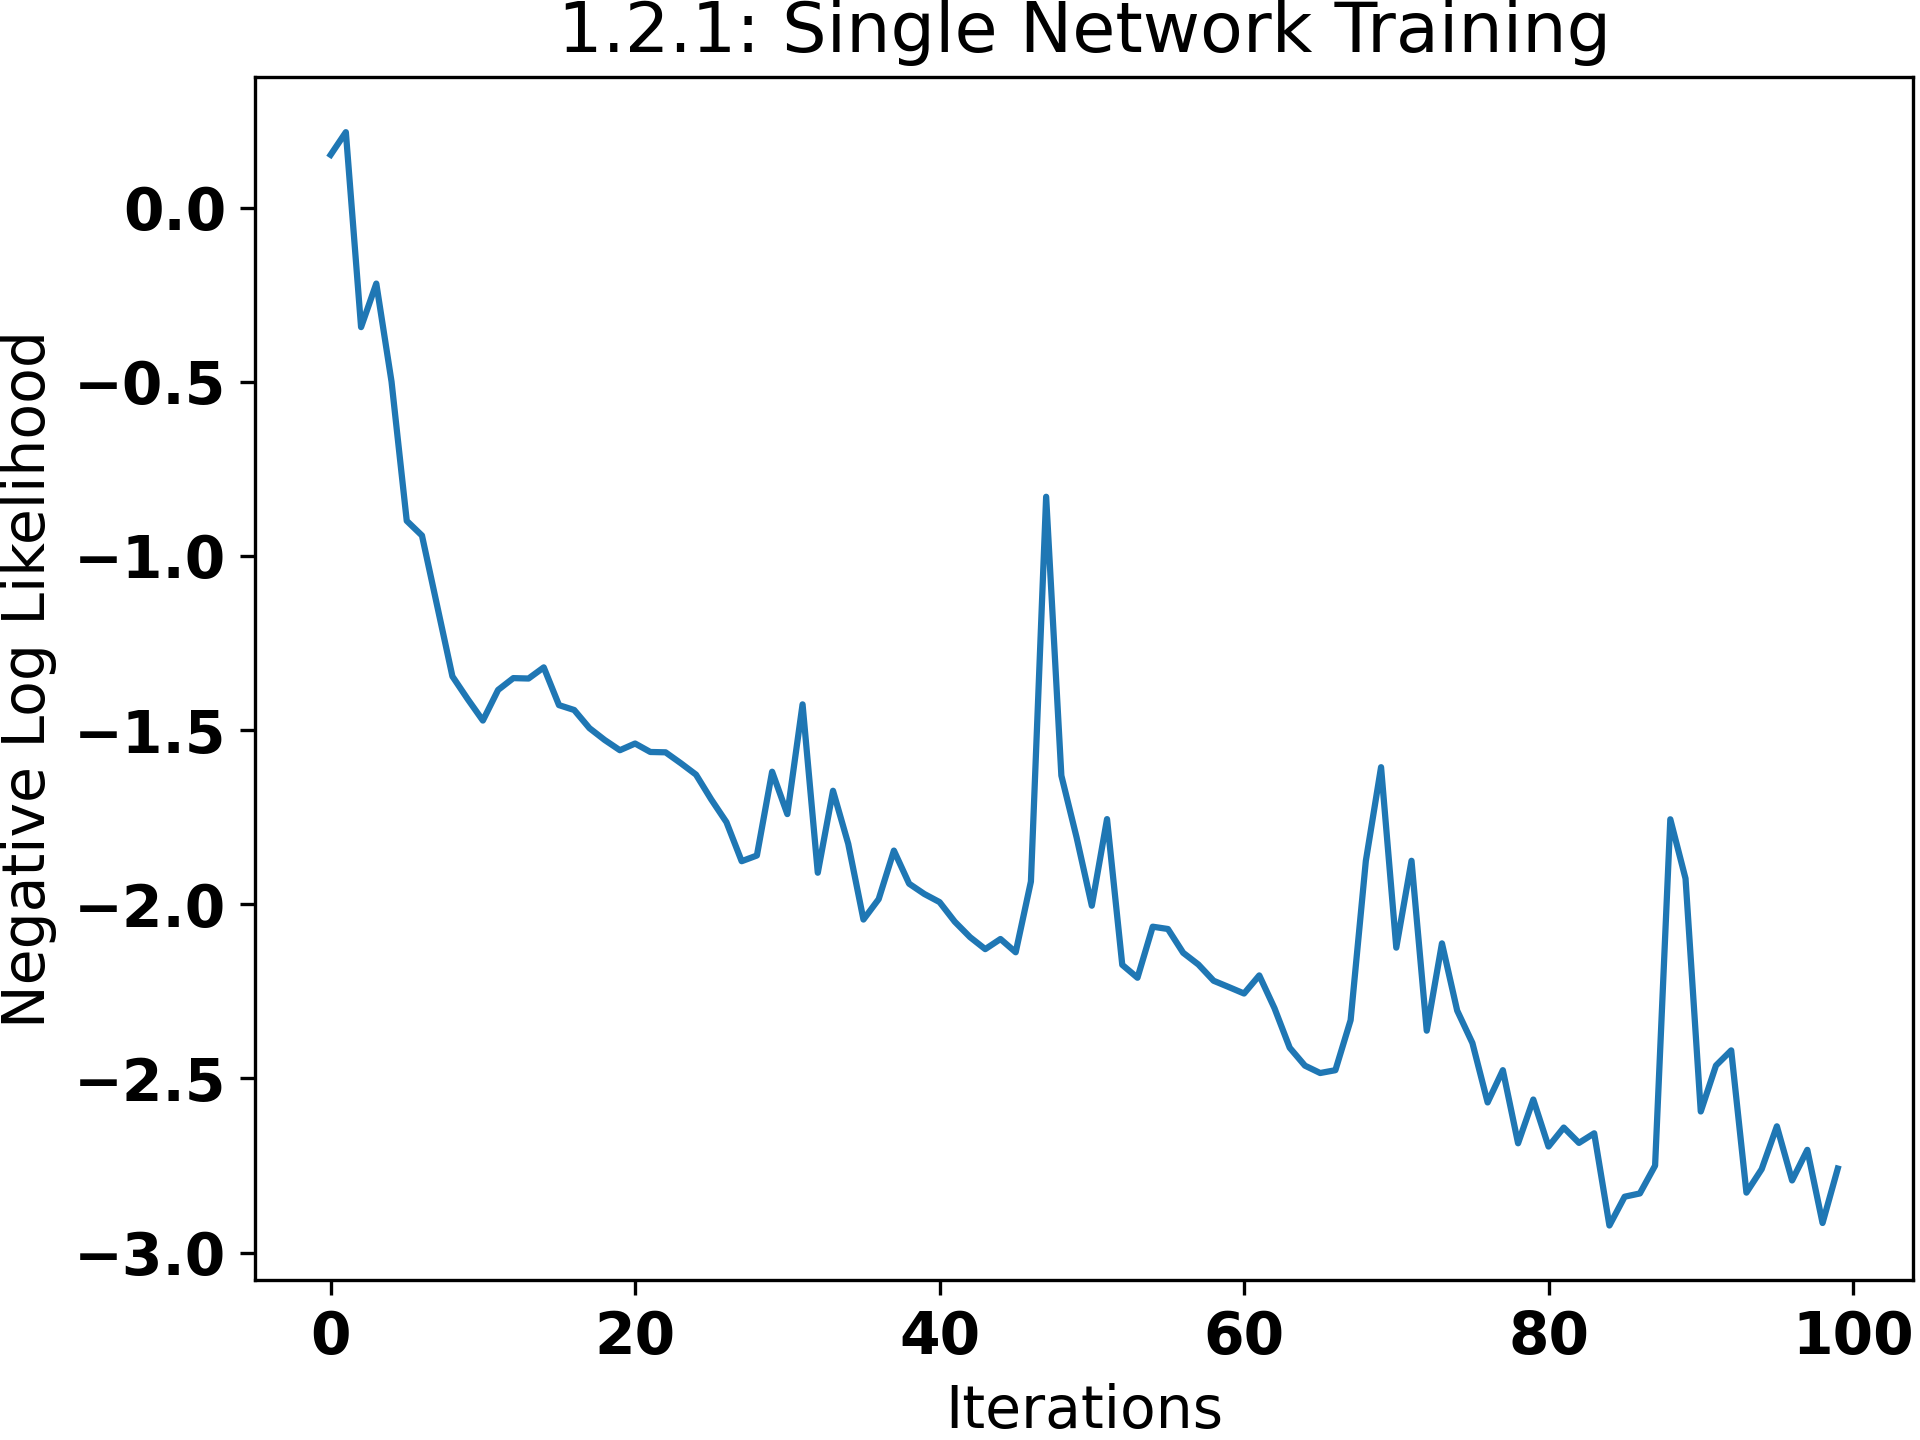
\includegraphics[width=0.8\linewidth]{1.2.1-loss.png}
        \label{fig:placeholder}
    \end{figure}
\end{center}
\end{tcolorbox}

\subsection*{1.2.2 MPC with random sampling (10 pt)}

Success percentage
\begin{tcolorbox}[fit,height=1cm, width=5cm, blank, borderline={1pt}{1pt},nobeforeafter, valign=center]
\begin{center}
     \large{24\%}
\end{center}
\end{tcolorbox}

\subsection*{1.2.3 MPC with CEM (10 pt)}

Success percentage
\begin{tcolorbox}[fit,height=1cm, width=5cm, blank, borderline={1pt}{1pt},nobeforeafter, valign=center]
\begin{center}
    \large{36\%}
\end{center}
\end{tcolorbox}

\subsection*{1.2.4 Random sampling vs. CEM  (6 pt)}

\begin{tcolorbox}[fit,height=15em, width=40em, blank, borderline={1pt}{1pt},nobeforeafter, valign=center]
\begin{center}
CEM outperforms random action by more intelligently selecting action sequences that lead to higher success rates. CEM + MPC didn't perform great in the recorded performance, achieving a success rate of only 36\%. However, on varying runs, it shows promise. The derived policy fails when it sees out-of-distribution state-action pairs. Our single probabilistic model starts to predict inaccurate transitions, and this error amplifies over longer horizons.
  
\end{center}
\end{tcolorbox}


\subsection*{1.3 MBRL with PETS (15 pts)}

\subsection*{1.3.1 Training loss plot (10 pt)}

\begin{tcolorbox}[fit,height=30em, width=40em, blank, borderline={1pt}{1pt},nobeforeafter]
\begin{center}
    \begin{figure}[H]
        \centering
        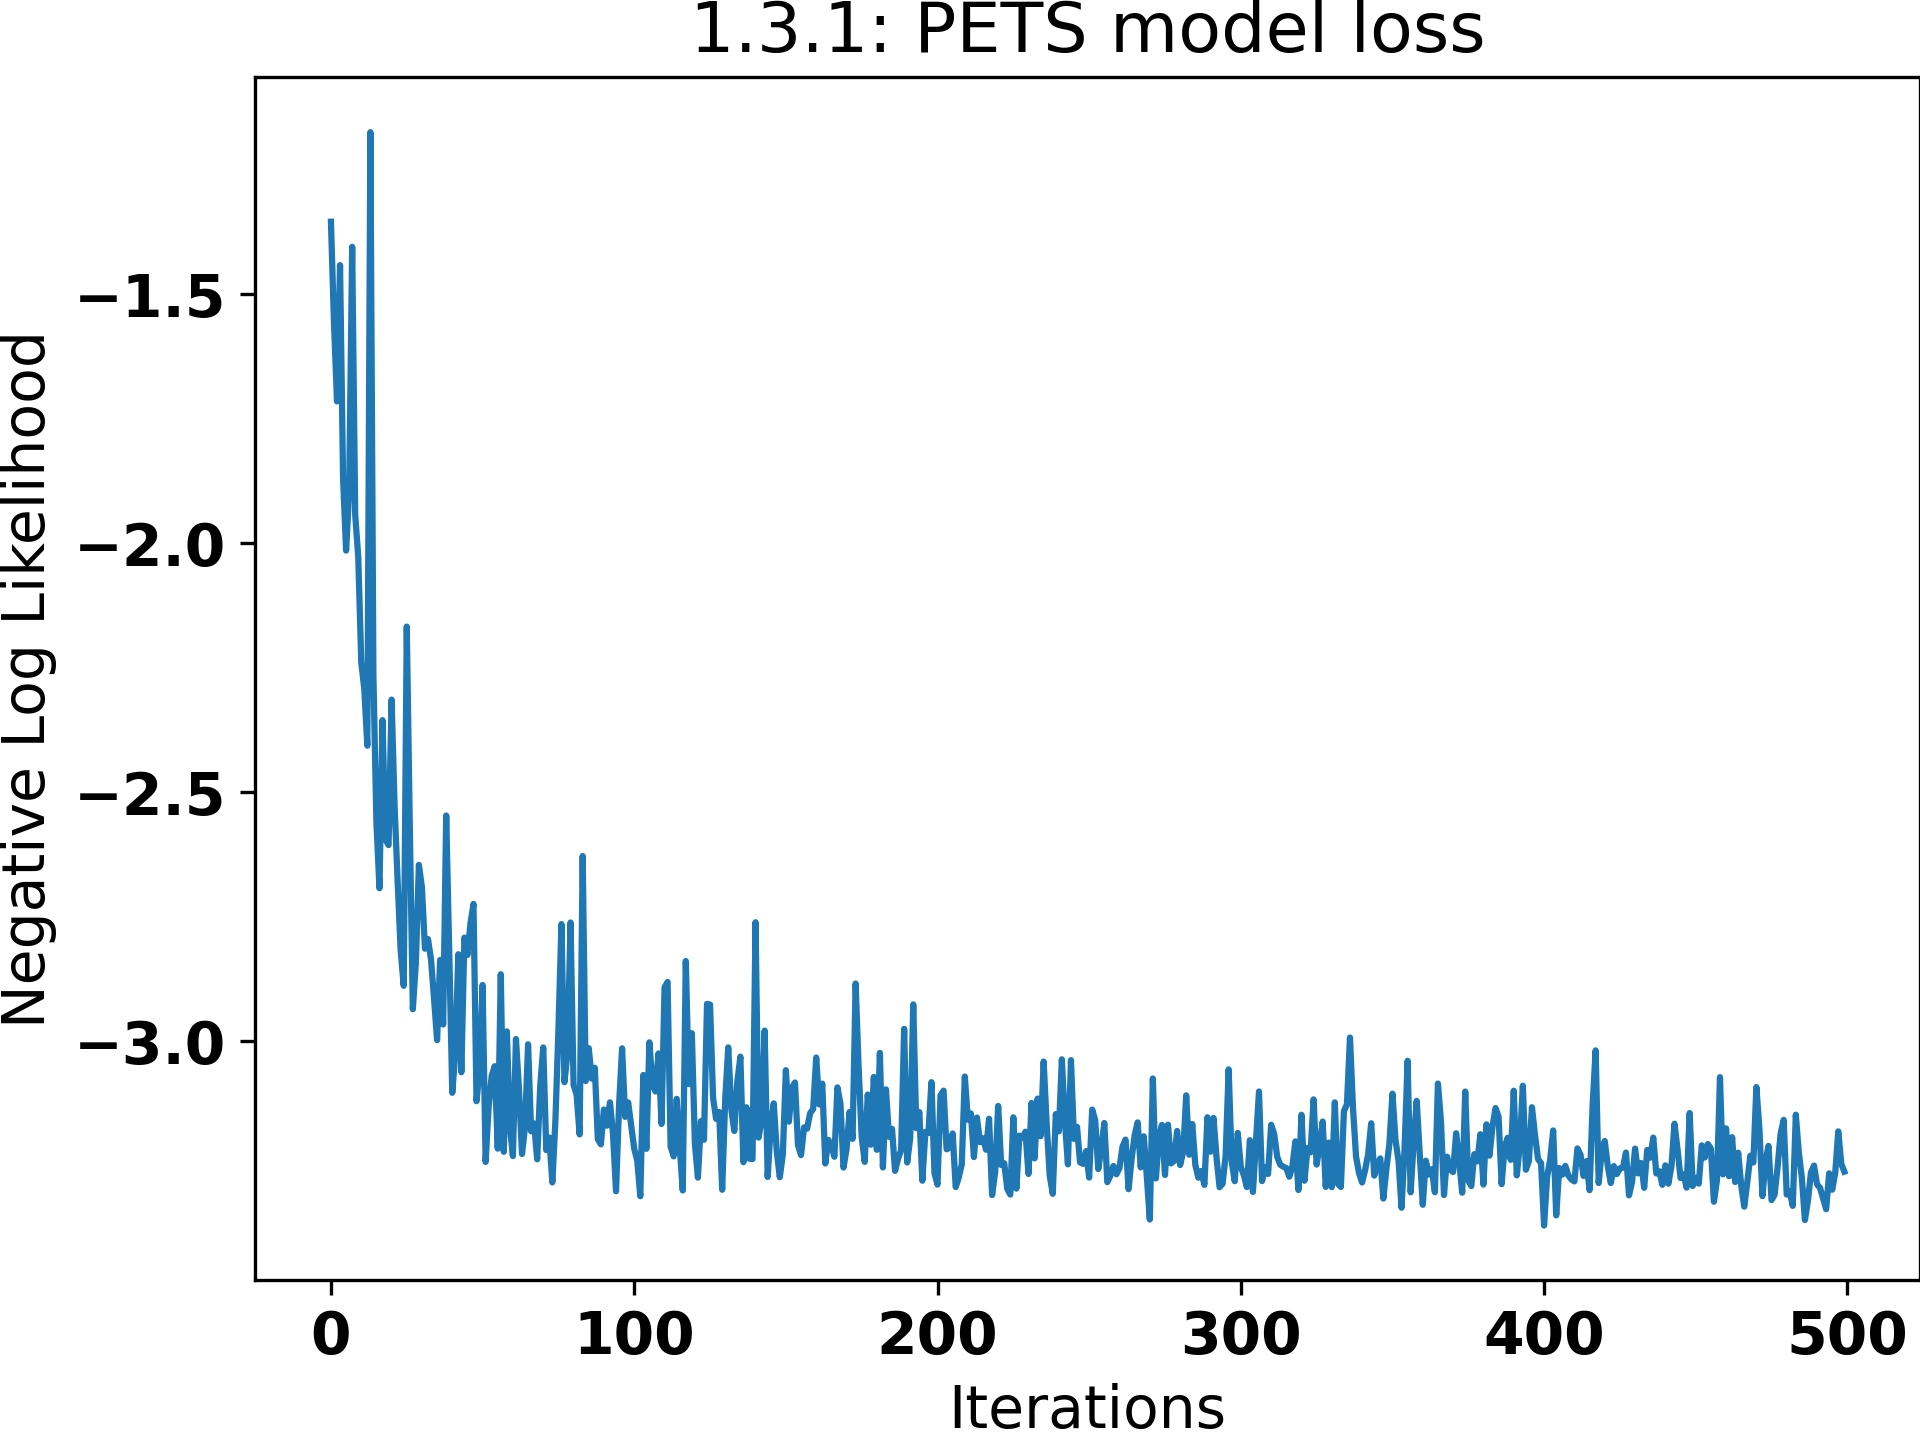
\includegraphics[width=0.8\linewidth]{1.3.1-loss.png}
        \label{fig:placeholder}
    \end{figure}
\end{center}
\end{tcolorbox}

\subsection*{1.3.2 Test percentage of successes plot (5 pt)}

\begin{tcolorbox}[fit,height=30em, width=40em, blank, borderline={1pt}{1pt},nobeforeafter]
\begin{center}
    \begin{figure}[H]
        \centering
        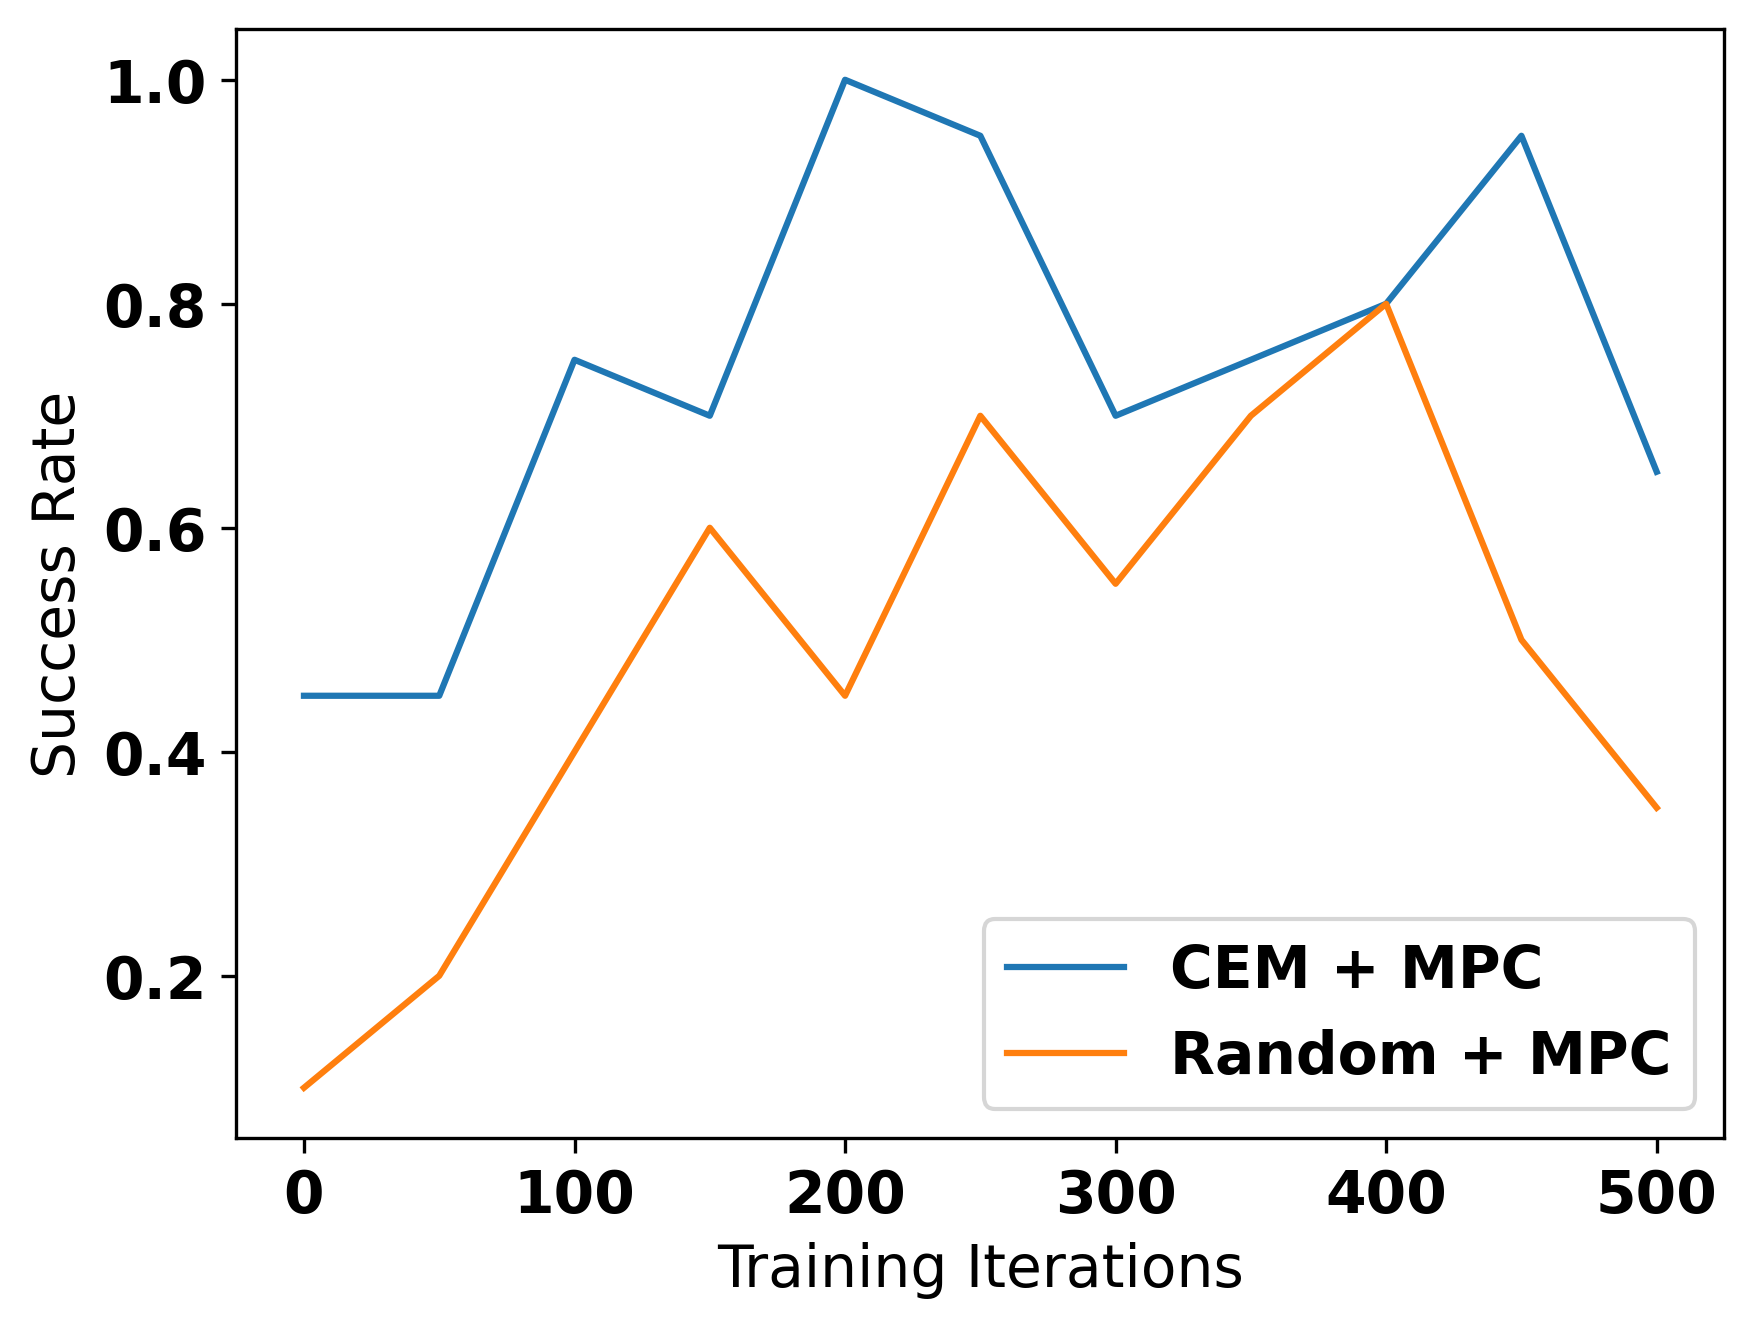
\includegraphics[width=0.8\linewidth]{2-cem-vs-random-Success Rate.png}
        \label{fig:placeholder}
    \end{figure}
\end{center}
\end{tcolorbox}

\subsection*{1.4 Training with synthetic data (30 pts)}

\subsection*{1.4.1 Ablation over model vs real data (10 pt)}
\begin{tcolorbox}[fit,height=30em, width=40em, blank, borderline={1pt}{1pt},nobeforeafter]
\begin{center}
     \begin{figure}[H]
        \centering
        \includegraphics[width=0.8\linewidth]{1.4.1-synthetic_ratio_success_rate.png}
        \label{fig:placeholder}
    \end{figure}
\end{center}
\end{tcolorbox}

\subsection*{1.4.2 Ablation over the rollout lengths (10 pt)}

\begin{tcolorbox}[fit,height=30em, width=40em, blank, borderline={1pt}{1pt},nobeforeafter]
\begin{center}
     \begin{figure}[H]
        \centering
        \includegraphics[width=0.8\linewidth]{1.4.2-rollout_length_success_rate.png}
        \label{fig:placeholder}
    \end{figure}
\end{center}
\end{tcolorbox}

\subsection*{1.4.3 Model error over rollout lengths (10 pt)}

\begin{tcolorbox}[fit,height=30em, width=40em, blank, borderline={1pt}{1pt},nobeforeafter]
\begin{center}
     \begin{figure}[H]
        \centering
        \includegraphics[width=0.8\linewidth]{1.4.3-l2_error_rollout.png}
        \label{fig:placeholder}
    \end{figure}
\end{center}
\end{tcolorbox}

\subsection*{1.4.4 MBRL vs Policy Gradient (5pt)}

\begin{tcolorbox}[fit,height=30em, width=40em, blank, borderline={1pt}{1pt},nobeforeafter, valign=center]
\begin{center}
    MBRL is more preferable when sample efficiency and fast adaptation are important, as it uses a learned model to simulate and plan without excessive "real world" interaction. It also excels in tasks requiring planning and foresight. Policy gradients are preferred when modeling the environment is difficult or infeasible, especially in high-dimensional or complex action spaces.
\end{center}
\end{tcolorbox}

\clearpage
\section*{Feedback}

\textbf{Feedback}: You can help the course staff improve the course for future semesters by providing feedback. You will receive a point of you provide actionable feedback. What was the most confusing part of this homework, and what would have made it less confusing?
\begin{solution}[height=4cm, valign=center]
The documentation could be made a lot easier to follow with a clearer structure and consistent numbering. It sometimes felt confusing to jump between parts because it wasn’t always obvious how the sections connected. A bit more organization and a smoother flow could help.
\end{solution}

\textbf{Collaboration}: Detail the work division amongst your group below.
\begin{solution}[height=4cm]

All members contributed equally. We worked on different parts of the code separately, but regularly discussed and helped each other fix bugs. 

\end{solution}

\noindent\textbf{Time Spent}: How many hours did you spend working on this assignment? Your answer will not affect your grade. Please average your answer over all the members of your team.
\begin{solution}[height=4cm]
\begin{table}[H]
    \centering
    \begin{tabular}{r|c}
        Alone &  \hspace{3em} 6
        \\ \hline
        With teammates & \hspace{3em} 2
        \\ \hline
        With other classmates & \hspace{3em} 0
        \\ \hline
        At office hours & \hspace{3em} 2
        \\ \hline
    \end{tabular}
\end{table}
\end{solution}

\end{document}